%; whizzy chapter
% -initex iniptex -latex platex -format platex -bibtex jbibtex -fmt fmt
% 以上 whizzytex を使用する場合の設定。

%     Kansai Debian Meeting resources
%     Copyright (C) 2007 Takaya Yamashita
%     Thank you for Tokyo Debian Meeting resources

%     This program is free software; you can redistribute it and/or modify
%     it under the terms of the GNU General Public License as published by
%     the Free Software Foundation; either version 2 of the License, or
%     (at your option) any later version.

%     This program is distributed in the hope that it will be useful,
%     but WITHOUT ANY WARRANTY; without even the implied warranty of
%     MERCHANTABILITY or FITNESS FOR A PARTICULAR PURPOSE.  See the
%     GNU General Public License for more details.

%     You should have received a copy of the GNU General Public License
%     along with this program; if not, write to the Free Software
%     Foundation, Inc., 51 Franklin St, Fifth Floor, Boston, MA  02110-1301 USA

%  preview (shell-command (concat "evince " (replace-regexp-in-string "tex$" "pdf"(buffer-file-name)) "&"))
% 画像ファイルを処理するためにはebbを利用してboundingboxを作成。
%(shell-command "cd image200708; ebb *.png")

%%ここからヘッダ開始。

\documentclass[mingoth,a4paper]{jsarticle}
\usepackage{kansaimonthlyreport}
\usepackage[dvips]{xy}
\usepackage{ascmac}

% 日付を定義する、毎月変わります。
\newcommand{\debmtgyear}{2010}
\newcommand{\debmtgdate}{23}
\newcommand{\debmtgmonth}{05}
\newcommand{\debmtgnumber}{35}

\begin{document}

\begin{titlepage}

% 毎月変更する部分、本文の末尾も修正することをわすれずに

 第\debmtgnumber{}回 関西 Debian 勉強会資料

\vspace{2cm}

\begin{center}
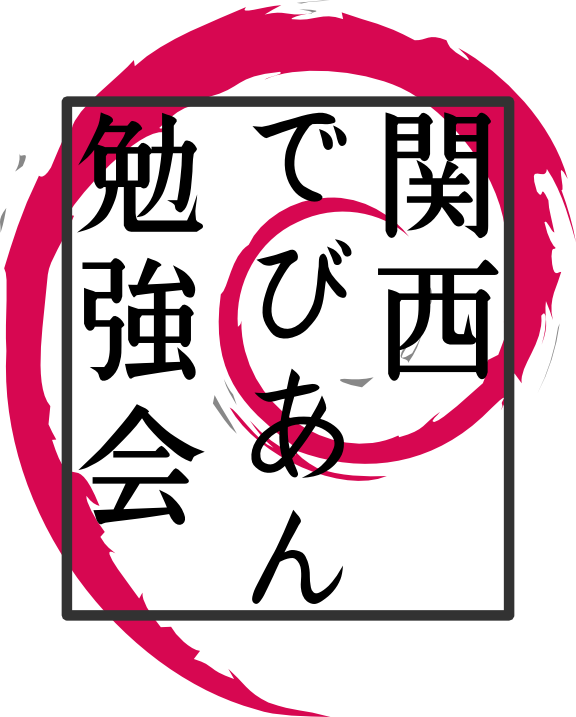
\includegraphics{image200802/kansaidebianlogo.png}
\end{center}

\begin{flushright}
\hfill{}関西 Debian 勉強会担当者 佐々木・倉敷・のがた \\
\hfill{}\debmtgyear{}年\debmtgmonth{}月\debmtgdate{}日
\end{flushright}

\thispagestyle{empty}
\end{titlepage}

\dancersection{Introduction}{Debian JP}

\subsection*{}%ロゴ用のスペース稼ぎ
 
関西 Debian 勉強会はDebian GNU/Linux のさまざまなトピック(新しいパッケー
ジ、Debian 特有の機能の仕組、Debian 界隈で起こった出来事、などなど)に
ついて話し合う会です。

目的として次の三つを考えています。
\begin{itemize}
      \item MLや掲示板ではなく、直接顔を合わせる事での情報交換の促進
      \item 定期的に集まれる場所
      \item 資料の作成
\end{itemize}

それでは、楽しい一時をお楽しみ下さい。

\clearpage

\begin{minipage}[b]{0.2\hsize}
 {\rotatebox{90}{\fontsize{80}{80}
{\gt 関西デビアン勉強会}}}
\end{minipage}
\begin{minipage}[b]{0.8\hsize}
\hrule
\vspace{2mm}
\hrule
\setcounter{tocdepth}{1}
\tableofcontents
\vspace{2mm}
\hrule
\end{minipage}

\dancersection{事前課題}{のがたじゅん}

5月の事前課題はSqueezeとubuntuの発表ということで、両者の使った感じについ
て尋ねてみました。

\begin{enumerate}
 \item Squeezeを使っていますか? 使った感じはどうですか? 
 \item Lucid Lynxを使っていますか? 使った感じはどうですか?
\end{enumerate}

申し込みをされた方の回答は以下になります。

\iffalse
\begin{prework}{ ichinomoto }

1.Squeezeは使用していません。
debian系を使い出したのはUbuntu9.10からで、それまではPlamoLinuxをメインで使っていたためです。

2.Lucid Lynxは使っています。
VM上でですが、起動が速いのとハードの自動認識などデフォルトでなんでも設定が完了しているのがすばらしい。

すみません、土曜日の仕事の状況によっては最初から参加できない可能性がありますが大丈夫でしょうか?

案の定仕事の方が押してきて参加が無理になってしまいました…
ぎりぎりで参加の申し込みとキャンセルになってしまい大変申し訳ありません。


\end{prework}
\fi


\begin{prework}{ dictoss(杉本 典充) }

    \begin{enumerate}
          \item sidを少しずつ使い出したので、Squeezeには手が届いてないです。これから使ってみます。
          \item Lucid Lynx(というかUbuntu自体)はまだ使ったことがないです。
    \end{enumerate}

\end{prework}


\begin{prework}{ 山田 洋平 }
    \begin{enumerate}
          \item Squeeze を使っています。というかずっと testing ばかり使っていて、Lenny がどんなだったか覚えてません...
          \item Lucid Lynx はまだ使っていませんが、去年から Ubuntu も、使い始めました。せっかくなので持って行きます。
    \end{enumerate}

\end{prework}



\begin{prework}{ かわだてつたろう }

    \begin{enumerate}
          \item 
使っています。
普段主に使う用途(Web と Mail)では全く不便は感じません。
更新が頻繁に行われるので出先で aptitude safe-upgrade するハメになると泣けます。
  \item 
使っていません。
    \end{enumerate}

\end{prework}



\begin{prework}{ ikuya }
    \begin{enumerate}
          \item 
        玄柴で使っています。とてもいい感じです。
          \item 
        レッツノートやテスト環境で使っています。非常に素晴らしいです!
    \end{enumerate}

\end{prework}



\begin{prework}{ 山下康成@京都府向日市 }
    \begin{enumerate}
          \item 使ってません(滅
          \item 使ってません(亡
    \end{enumerate}
\end{prework}



\begin{prework}{ 西山和広 }

    \begin{enumerate}
          \item 
        VMwareでsidをサーバ的にsshで入って使っていますが、pamでupdate-motdが呼ばれるようになっているなど、Ubuntuから取り込まれたものがあったり、順調にソフトウェアのバージョンが上がっていたりして無難にバージョンが上がっているという感じがします。
          \item 
        Gwibberの挙動がよくわからなかったり、標準のテーマだとemacsで警告が出て使いにくかったり、rubyのビルドがGccSspでひっかかったりするなど、微妙なところはあるけれど、普段使う範囲ではあまり困らない感じです。
    \end{enumerate}

\end{prework}



\begin{prework}{ 0xBCD1BC92 (yabuki.yukiharu) }

    \begin{enumerate}
          \item 
        Debianのtestingは使ってません。stableかunstableしか使ってません。身体が弱くなったので宴会には参加できません。すいません。
          \item 
        Ubuntuの10.04は使ったことがありません。
    \end{enumerate}
\end{prework}



\begin{prework}{ 榎真治 }

    \begin{enumerate}
          \item 使っていません
          \item そのうちインストールしてみるつもりです
    \end{enumerate}
\end{prework}



\begin{prework}{ google-account@rolf.leggewie.biz }

できるだけ参加したいと思います。

\end{prework}



\begin{prework}{ のがたじゅん }

    \begin{enumerate}
          \item すみません。お題を出したのにsid使ってます…。%
          \item
        使ってみました。見た目が綺麗ですね。KMSでハマっている人多いみたいですね。半年前の自分を見ているようです
    \end{enumerate}
\end{prework}

\begin{prework}{ ohachige }
    \begin{enumerate}
          \item 
        Debian sid を職場で使っています。
        いいと思います。
          \item 
        家の3台のPCをアップグレードしました。
        1台だけウィンドウのボタンが右側のままで、なんか変な気がしますが、それ以外は問題なくアップグレードできました。
        iPod Touch の中身が見れるようになったのはうれしいです。
    \end{enumerate}
\end{prework}



\begin{prework}{ IPv6waterstar }

両者とも使ってません。
\end{prework}



\begin{prework}{ lurdan }

    \begin{enumerate}
          \item 10日未来の squeeze を使っています。いつも通りです。
          \item
        リリース直前に試して、いろいろ挫折しました。デスクトップ用途だったらいい出会いになっていたかもね……
    \end{enumerate}
\end{prework}



\begin{prework}{ Takashi Nakamoto }

無回答

\end{prework}



\begin{prework}{ 中川舟(しゅう) }
    \begin{enumerate}
          \item 
        まだDebian lennyを使用して2ヶ月なので、
        Squeezeは使っていません。
          \item 
        初めて知りました!
        使った事はありません。
    \end{enumerate}
\end{prework}

\begin{prework}{ kazken3 }

無回答

\end{prework}

\dancersection{最近のDebian関係のイベント報告}{Debian JP}

\subsection{前回の関西Debian勉強会}

前回の関西Debian勉強会は, 4 月 25 日に大阪港区民センターで行なわれました.
山下@京都府向日市さんによる正規表現講座と,
佐々木による(ゆるい)Debian でのデスクトップ環境に関するお話しでした.
%
正規表現に関しては, 簡単な所で意外とハマっている人がいたりして, 大変勉強になりました.
デスクトップ環境については, 
山田さんがタイル型マネージャを使っていることが判明したり,
杉本さんの Desktop を見て「タイルで良いじゃん!」というツッコミが入ったり,
想定していた以上に盛り上がりました\footnote{%
タイル型マネージャについては, 
そのうち倉敷さんが xmonad の布教をすると思いますので,
皆さま楽しみにしていて下さい(笑).}.

\subsection{第 64 回東京 Debian 勉強会}

5 月 15 日, 第 64 回東京 Debian 勉強会が開催されました.
今回は「つくらぐ(筑波大学 Linux Users Group)」さんとの合同で, 筑波大学で
開催されました.
当日の様子は

\subsection{オープンセミナー2010@岡山参加報告}

5月15日岡山県立大学で開催された「オープンセミナー2010@岡山」で、「次期リ
リース Debian 6.0(コード名: Squeeze)を見る」というタイトルで、のがたじゅ
んがSqueezeの状況について発表してきました。

15分の短い時間でしたが、やまねさんが発表された「Squeeze について思いを巡
らせてみる」と佐々木さんが発表された「次期リリースのDebian 6.0(コード
名:Squeeze)を見てみよう」をベースに、5月時点でのSqueezeの情報と、先日アナ
ウンスのあったundefomaによるTeXまわりの影響と日本語manについて話をしてき
ました。

自分としてはうまく説明できたか不安でしたが、アンケート\footnote{アンケー
ト集計結果 - オープンセミナー2010@岡山:
\url{http://openseminar.okaya.ma/2010/wiki.cgi?page=\%A5\%A2\%A5\%F3\%A5\%B1\%A1\%BC\%A5\%C8\%BD\%B8\%B7\%D7\%B7\%EB\%B2\%CC}}
やTwitter\footnote{ Togetter - まとめ「オープンセミナー2010@岡山
(2010.5.15)」: \url{http://togetter.com/li/21450}}の反応を見ると、おお
むね好評だったようでです。

岡山県立大学の情報通信工学科の演習室ではDebianが動いているそう
\footnote{「情報通信工学科の演習室でDebian GNU/Linuxが動いている3つ(くら
い)の理由」荒井 剛(岡山県立大学):
\url{http://openseminar.okaya.ma/2009/wiki.cgi?page=\%B8\%F8\%B3\%AB\%BB\%F1\%CE\%C1&file=OS2009LT\%2Dtarai\%2Epdf&action=ATTACH}}
ですし、また機会があれば岡山方面にもお話しをしたいと思います。
また, 
セミナーの様子が動画で公開されています。\footnote{次期リリース Debian
6.0(コード名: Squeeze)を見る: \url{http://peevee.tv/v?6ne552}}

\dancersection{Debianユーザのための Ubuntu 入門}{あわしろいくや}

\subsection{自己紹介}

\begin{itemize}
      \item Ubuntu Japanese Team: 日本語入力担当(らしい)
      \item OpenOffice.org 日本ユーザ会
      \item Debian では scim-anthy とかのメンテナ(最近は任せきり)
      \item Anthy もリリースしてた(今はやる気がなくて困り中)
      \item 雑誌とかに原稿書いたり
      \item 本業も微妙に Ubuntu
\end{itemize}

\subsection{Ubuntu はやわかり}
\begin{itemize}
      \item Linuxディストリビューション\\
    $leftrightarrow$ Debianはユニバーサルオペレーティングシステム
      \item アーキテクチャはi386/AMD64/ARM(非公式にはIA64とかPowerPCとか)
      \item 半年に1度リリース, 2年に1度LTS(Long Term Support)がリリース
      \item GNOME採用, 格好いいアートワーク...
      \item 運営はCanonicalを主体としたコミュニティ. DDもたくさん
      \item CD1枚に収まるサイズでライブCD(DVDもあるけどね)
      \item たくさんの派生版: KubuntuとかNetbook Editonとか(非公式なものもたくさん)
      \item サーバ版もある: 簡単にクラウド環境をセットアップ
      \item リポジトリ
    \begin{itemize}
          \item main: Canonicalによってメンテナンスされる. デフォルトでインストールされる
          \item universe: コミュティによるメンテナンス
          \item multiverse: Debianでいうところのnon-free
          \item restricted: プロプライエタリなドライバ
    \end{itemize}
      \item Alternate CD: CUIインストーラ. アップグレードにも使える
      \item Ubuntu Netbook Editon: 専用UI
\end{itemize}

\subsection{Launchpadってなに?}
\begin{itemize}
      \item やたら高性能なCMS\\
     →BTS, 翻訳, アイディアの集積, Q\&A
    開発プロジェクトのホスティング, Personal Pachage Archive
      \item これのアカウントを取ることによって、Ubuntu Oneとかも使用可能になる
\end{itemize}

\subsection{Ubuntu Oneってなに?}
\begin{itemize}
      \item Dropboxみたいなファイル同期サービス\\
    2GBまで無料。50GBまで月10ドル. TomboyとかFirefoxのブックマークも同期.
    Ubuntu One Music Storeで買った曲もUbuntu Oneに転送される
\end{itemize}

\subsection{LTSってなに?}
\begin{itemize}
      \item Long Term Support: 通常はリリース後18ヶ月サポート
      \item LTSはデスクトップ版で3年、サーバ版で5年サポート
      \item LTSはポイントリリースあり: Ubuntu 10.04.1とか
      \item LTS→LTSのアップグレードもサポート.
\end{itemize}

\subsection{コードネームとバージョニング}
\begin{itemize}
      \item  動詞+動物. 頭韻を踏む: Lucid Lynxとか、Maverick Meerkatとか. LL→MM. 
    https://wiki.ubuntu.com/DevelopmentCodeNamesに予想とか書いてあって笑える
    \item バージョンはリリース年+月. 
\end{itemize}

\subsection{デスクトップ版}

\begin{itemize}
      \item Ubuntu 10.04,
      \item Ubuntu Netbook Editon 10.04, 
      \item Kubuntu 10.04 LTS, 
      \item Kubuntu Netbook Remix, 
      \item Xubuntu 10.04, 
      \item Lubuntu 10.04 (非公式)
\end{itemize}

\subsection{サーバ版}

\begin{itemize}
      \item Ubuntu Server: 専用のインストーラが用意. Xなし
      \item 通常のサーバと、Ubuntu Enterprise Cloud(Eucaliptus)のセットアップ
      \item LTS → サポート期間が長い
      \item Byobu: screen用のプロファイル
      \item インストールの最初で、Ubuntu ServerかUECを選択する
    →
    Ubuntu Serverを選択すると、具体的に何をインストールするか聞かれる
\end{itemize}

\subsection{Ubuntu 10.04 LTSの概要}
\begin{itemize}
      \item 3番目のLTS
      \item Ubuntu One Music Store(MP3の音楽が買える)
      \item 起動時間の短縮(5秒切るとか)
      \item Noueveau(ぬーぼー): NVIDIA用のオープンそーすなドライバ
      \item GIMPサヨウナラ: F-Spotで簡単なレタッチならできるという理屈
      \item PiTiViコンニチハ: 動画編集ソフト
      \item GWibberコンニチハ:  Twitterクライアント
      \item ウィンドウ・マネージャのボタンの位置: 左に移った
      \item テーマの変更
      \item フォントの変更: Takaoフォント
      \item ARMの話
    \begin{itemize}
          \item Ubuntu 9.04まではARMv5でビルド
          \item 9.10ではカーネルのみARMv7でビルド: Sheevaplugで動かない
          \item 10.04ではユーザランドもARM7でビルドとか $\rightarrow$ Debianの出番だ!
    \end{itemize}
\end{itemize}

\subsection{Ubuntuの活用事例}
\begin{itemize}
      \item NetWalker
      \item SheevaPlug
      \item Dell Inspiron Mini10 $\rightarrow$  あろうことか10.04で廃止
\end{itemize}

\subsection{Ubuntuの歴史}

\begin{itemize}
      \item 2004年、Mark Shuttleworthとオープンソース開発者が集まって準備開始
    \begin{itemize}
          \item タイムベースリリース
          \item Debianベース, GNOME
          \item 自由へのコミットメント
    \end{itemize}
      \item 最初のリリースはUbuntu 4.10, 最初に日本語サポートが入ったのは6.06
\end{itemize}

\subsection{Debianとの関係}
\begin{itemize}
      \item まあまあ良好? メンテナが同じパッケージも多い(IBusとか)
      \item universeはunstableあるいはtestingのパッケージからインポート
      \item 最近は、まずDebianのリポジトリに入ることも多いらしい。
      \item Ubuntuの人たちがDebianのバグを潰したり
      \item もともと10.04はSqueezeと同時期リリースの予定だった
    \begin{itemize}
          \item 10.04ではtestingからのインポートで、bug squashの手伝いになるというもくろみもあったらしい
    \end{itemize}
    \item Debian向けのパッチも公開. 
  パッチの共用化\footnote{\url{https://wiki.ubuntu.com/UbuntuDevelopment/PatchTaggingGuidelines}}
\end{itemize}


\subsection{Debian との違い}
\begin{itemize}
      \item 言語サポート: 各言語ごとに言語パックを準備
      \item 日本語入力: ibus 
      \item ードウェア・ドライバ: ビデオカードとか無線LANのプロプライエタリなドライバを簡単にインストール
      \item Mozillaから正規にライセンスされている(らしい)
\end{itemize}

\subsection{開発スタイル}
 
  \begin{itemize}
        \item まずスケジュールを立てる
        \item みんなでがんばる
        \item 開発版と称してスナップショットをリリース
        \item スケジュールは、前のバージョンのリリース前に、コードネームと一緒に発表
        \item リリース後にUDSというミーティングを開いて、何をするか決める
        \item リリース後にUDSというミーティングを開いて、何をするか決める
        \item LaunchpadのBlueprintsに、概要や重要性や進捗を書く\\
      \url{https://blueprints.launchpad.net/ubuntu/maverick}
  \end{itemize}

  \subsection{Debianの方が優れているところ}
  \begin{itemize}
        \item headのおっかけ: sidとかexperimentalとか
        \item Ubuntuだと半年に一度変更しないとダメ.
        \item 最小構成でのインストール
        \item いちおうminimalはあるが,
      基本的にはメタパッケージベース
  \end{itemize}


  \subsection{さらなる情報}
  \begin{itemize}
        \item Software Design 6月号(書いたのが結構前なので、情報がやや古い)
        \item ASCII.technologies 7月号
        \item アスキー・メディアワークス(福原遥ちゃんの表紙, 売り切れ必須!)
        \item うぶんちゅ!(CC-BY-SA) で公開
        \item Ubuntu Monthly Report (Software Design で執筆中. 
        \item 行っとけ! Ubuntu道場!(ASCII.jp で公開中)
  \end{itemize}
  

まとめ: 
今後も持ちつ持たれつ共存共栄でいきましょう!
というか、みんな好きなディストリビューション使えばいいよね


\dancersection{次期リリースの Squeeze を見てみよう}{のがたじゅん}

\subsection{はじめに}
5月の関西Debian勉強会はubuntu Japanese Teamのあわしろいくやさんがゲスト
ですので、Debianな人なら知ってることも改めて解説しながら、次期リリース予
定のSqueezeについて解説します。

\subsection{Squeezeって何?}
Squeezeとは次期リリース予定のDebian安定版の開発コードネームです。バージョ
ン番号は6.0です。Debianの開発コードネームは、映画Toy Storyのキャラクター
名から取られてて、Squeezeは3つ目のエイリアンです。

\subsection{いつリリースなの?}

去年7月に開催されたDebConf 9でリリースをタイムベース(時間で区切って)のリ
リースに移行することが発表されました。\footnote{Debian decides to adopt
time-based release freezes:
\url{http://lists.debian.org/debian-announce/2009/msg00009.html}}それによ
ると12月フリーズ(新規機能などの追加停止)、翌年3月にリリースの予定でした。

しかし、現安定版のLennyは2009年2月にリリースされ、まだ一年も経っていない
状況では早すぎるとの判断から、改めて2010年3月にフリーズに入る予定でした。
\footnote{Bits from the release team: Planning, request for help:
\url{http://lists.debian.org/debian-devel-announce/2009/10/msg00002.html}}

が、また一転。3月にネットワーク障害が起こったため、また仕切り直しになりフ
リーズは5月末から6月上旬に延期され\footnote{Bits from the Release Team:
Scheduling, transitions, how to help:
\url{http://lists.debian.org/debian-devel-announce/2010/04/msg00001.html}}
リリースは未定になっています。

\subsection{Squeezeのリリースゴール}
Squeezeのリリース目標ですが、現在のところ2009年に発表されたリリースゴール
から変わっていません。以下、Debianニュースの「Debian GNU/Linux 6.0
"Squeeze" リリースの目標」からの引用です。\footnote{Debian -- ニュース
-- Debian GNU/Linux 6.0 "Squeeze" リリースの目標:
http://www.debian.org/News/2009/20090730}

\begin{itemize}
 \item 多数のアーキテクチャサポートによる、64 ビットマシンへの 32 ビット
       パッケージのインストール事情の改善
 \item kFreeBSD サポート、Debian 初の non-linux アーキテクチャの導入
 \item dash を新しいデフォルトシェルとしてブート性能を改善し、 依存ベース
       のブートシステムによるブートプロセスのクリーンアップと 並行処理に
       よる性能向上を図る
 \item 品質保証 (QA) プロセスをさらに拡張してパッケージの品質向上につなげ
       る。その内容:
        \begin{itemize}
         \item 全パッケージについてクリーンインストール、アップグレード及
               び削除
         \item 基礎的な品質チェックに通らなかったパッケージの自動拒否
         \item ダブルコンパイルのサポート
        \end{itemize}
 \item 新しいパッケージ形式を策定して、 将来の開発の能率化と圧縮アルゴリ
       ズムの改善を図る
 \item 旧式のライブラリを削除してセキュリティを改善
 \item ipv6 の完全サポート
 \item ラージファイルのサポート
 \item アーカイブ全体の debug パッケージの自動生成。Google Summer of
       Code プロジェクトのインフラへの統合を保留しています。
 \item パッケージの長い説明を\"翻訳済みパッケージリスト\"に分離して翻訳を
       促進し、 また、組み込みシステム向けに小さくしたフットプリントを提
       供します。 小さくなった Packages ファイルに感謝します。
 \item パッケージに複数の属性をタグ付けするシステム、debtags の統合の改善
       によってパッケージ選択をもっと簡単に
 \item メンテナによりアップロードされたバイナリパッケージを破棄、再ビルド
       し、 制御下の環境でビルドされたパッケージだけを残す
\end{itemize}

\subsection{今、やることは?}

まだフリーズになってません。変更点があってもまだ間に合います。(といっても
大幅な変更は「5月21日までに連絡を」と言っていたので難しいかもしれませんが、
相談することが重要だと思います。)

それまでにRelease Critical Bug(リリースに障害となるバグ)を潰すこと、翻訳
を進めるなど、いろいろあります。

\subsection{日本語関連で注意しなければいけないこと}

まずDefomaを使わなくなったことによる影響があげられます。

DebianにはDefoma(Debian Font Manager)というフォントを独自で管理する仕組
みがありますが、現在メンテナンスされておらず外されることが決定しました。

デスクトップ環境ではFontconfigによるフォント管理があるのでDefomaが外さ
れても影響はありませんが、TeX環境、特に日本語TeX環境についてはDefomaに
機能を依存していたこともあり影響が出ることが確認されています。

日本語TeX環境での影響は、GhostScriptで日本語PostScriptが扱えない、
dvipsk-jaがビルドできない/使えないなどあります。

TeX以外では日本語manではmanの整形をするroff(groff)が日本語の文字に中途
半端な対応のため、きちんと整形して表示されないなどの問題が確認されてい
ます。

これらの問題について、先日、対応するテストパッケージとDebian JPのアナウン
スが出たので、ご協力いただける方はアナウンスを読んで、Debian JP Devel ML
で反応してください。\footnote{[debian-announce:00067] 「Squeeze」リリース
に向けて解決が必要なパッケージの開発・検証協力のお願い:
\url{http://lists.debian.or.jp/debian-announce/201005/msg00003.html}}

また、問題ではありませんが、武藤さんよりuimからibusへの変更の提案が
Debian JP Devel ML出されていて、意見を求めているので、関心のある方はご意
見などをお寄せください。\footnote{[debian-devel:17817] Re: 日本語タスク
(squeeze):
\url{http://lists.debian.or.jp/debian-devel/201005/msg00006.html}}

\dancersection{今後の予定}{Debian JP}

\subsection{次回の関西Debian勉強会}
次回、2010年6月の関西Debian勉強会は6月23日大阪福島区民センターでおこなう
予定です。現在決まっている予定は、「debhelper 7とcdbsについて」(佐々木)、
「今さら puppet ネタ」(倉敷) の 2 本です。

\subsection{オープンソースカンファレンス 2010 Kansai@Kyoto}
申し込みをしましたが、講師、ブースともに決まっていないので提案お待ちしています。



% 冊子にするために、4の倍数にする必要がある。
% そのための調整
\dancersection{メモ}{}
\mbox{}\newpage

\printindex
 \cleartooddpage

 \begin{minipage}[b]{0.2\hsize}
  \rotatebox{90}{\fontsize{80}{80} {\gt 関西デビアン勉強会} }
 \end{minipage}
 \begin{minipage}[b]{0.8\hsize}

 \vspace*{15cm}
 \rule{\hsize}{1mm}
 \vspace{2mm}
 
\includegraphics[width=2cm]{image200502/openlogo-nd.eps}
 \noindent \Large \bf Debian 勉強会資料\\ \\
 \noindent \normalfont \debmtgyear{}年\debmtgmonth{}月\debmtgdate{}日 \hspace{5mm}  初版第1刷発行\\
 \noindent \normalfont 関西 Debian 勉強会 (編集・印刷・発行)\\
 \rule{\hsize}{1mm}
 \end{minipage}

\end{document}
